\documentclass[../main.tex]{subfiles}

\begin{document}
\subsection{Linear Actuator} 
\label{linearActuator}
The linear actuator analysis is preformed to ensure that the holding force of the linear actuator generates a great enough friction to keep the gondola from moving. The analysis first solves for the acceleration in a scenario similar to that of worst case mention above in REF???? and in friction wheel slip section \ref{frictionSlip} with the the friction wheel motor not being powered, therefor the drive force $F_{Drive} = 0$. The inputs required to run this analysis are the geometry of the friction wheel, the motor, the hinge, the gondola, as well as the material properties of the braking surface, the mass of each gondola car, the maximum achievable thruster acceleration and the loading conditions specific to the worst case scenario. The sum of forces used to solve for the case are as follows. 
\begin{multline} \label{FxGondLA}
\Sigma F_{x} : (m_{1}+m_{2}) a_{x} + F_{NB3_{x}} + F_{NB4_{x}} =\\ \sin(\phi) (m_{1} + m_2)g + \cos(\beta) (m_1+m_2) a_{Thrust} + \frac{\sqrt{2}}{2} sin(\theta) F_{Spring}
\end{multline}
\begin{flalign} \label{FyGondLA}
\hspace{12pt}\Sigma F_{y} : F_{NB1_{y}} - F_{NB2_{y}} - F_{NB3_{y}} + F_{NB4_{y}} = \frac{\sqrt{2}}{2} F_{Spring} -\frac{\sqrt{2}}{2} F_{Spring} &&
\end{flalign}
\begin{multline} \label{FzGondLA}
\Sigma F_{z} : F_{NB1_{z}} + F_{NB2_{z}} + F_{NB3_{z}} + F_{NB4_{z}} =\\ \cos(\phi) (m_{1} + m_2)g - \frac{\sqrt{2}}{2} cos(\theta) F_{Spring} -\frac{\sqrt{2}}{2} F_{Spring} + \sin(\beta) (m_1+m_2) a_{Thrust}
\end{multline}

The braking force $F_{brake}$ must then be greater than the calculated acceleration $a_{x}$. The brake force is dependent on the friction force between the polyurethane and rubber contact piece of the linear actuator, as seen in Figure ???.  The breaking force is related to the linear actuator for $F_{LA}$ by the equation \ref{eqn:brake} below.
\begin{equation}
\label{eqn:brake}
F_{brake} = \mu_{braking surface} F_{LA}
\end{equation}

The value for $\mu_{braking surface}$ is based on the coefficient of friction between rubber and polyurethane which is 0.65 CITESTION???. Once the required linear actuator force is calculated it is compared with the Actuonix linear actuator in Appendix Datasheets \ref{LinAct} in order to make sure that the force is achievable.

\begin{figure}[H]
	\centering
	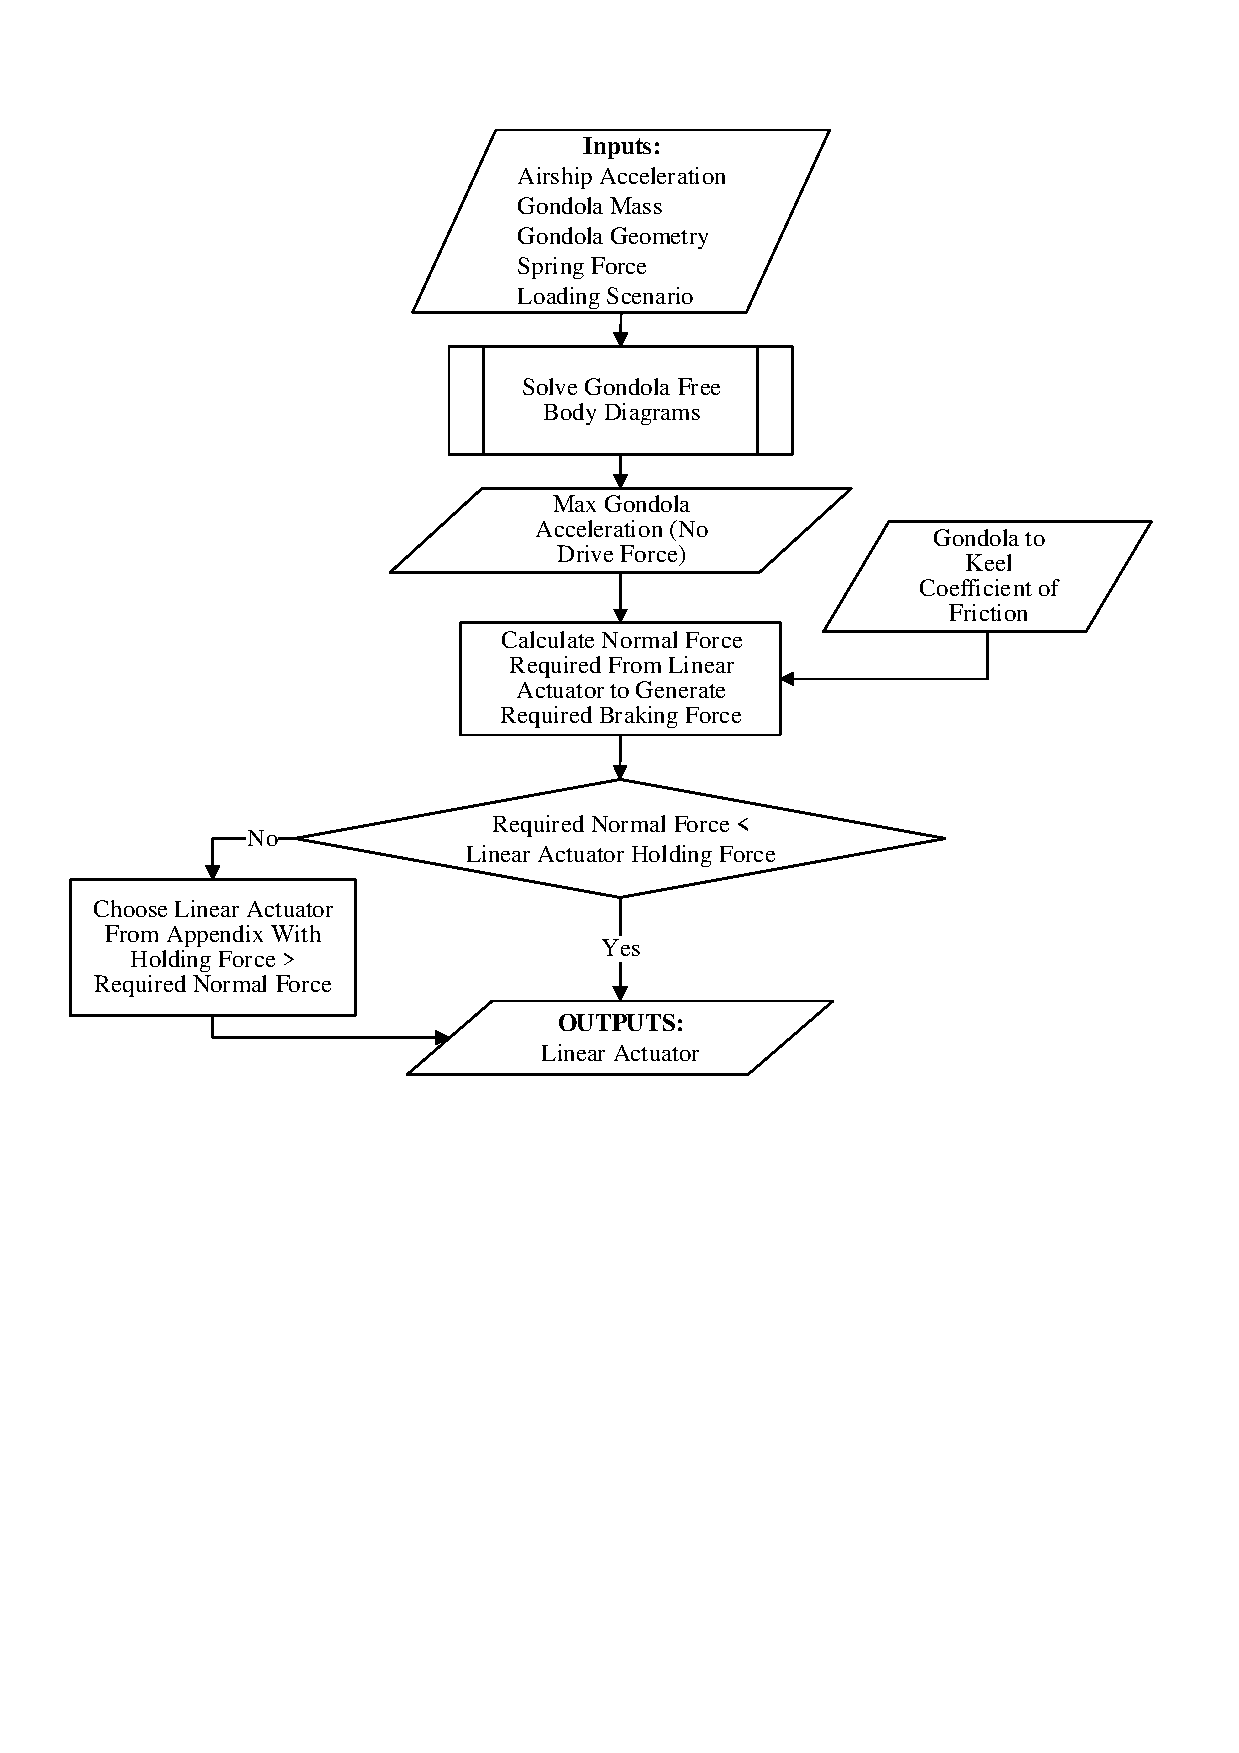
\includegraphics[width=\linewidth]{img/paramaterization/linearActuator.pdf}
	\caption{Parametrization Outline for the Bolt Compression}
	\label{fig:linearActuatorParametrization}
\end{figure}

\end{document}